\section{SEMILOGX Semilog X Axis Plot Function}

\subsection{Usage}

This command has the exact same syntax as the \verb|plot| command:
\begin{verbatim}
  semilogx(<data 1>,{linespec 1},<data 2>,{linespec 2}...,properties...)
\end{verbatim}
in fact, it is a simple wrapper around \verb|plot| that sets the
x axis to have a logarithmic scale.
\subsection{Example}

Here is an example of an exponential signal plotted first on a linear
plot:
\begin{verbatim}
--> y = linspace(0,2);
--> x = (10).^y;
--> plot(x,y,'r-');
\end{verbatim}


\centerline{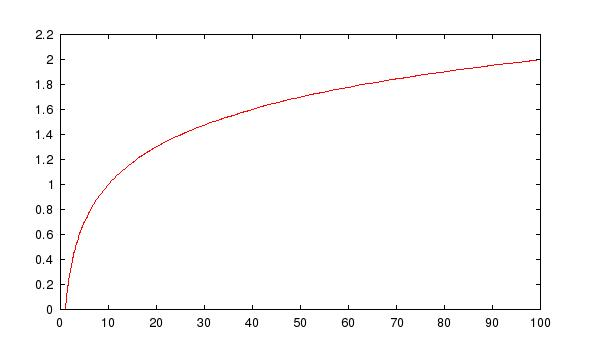
\includegraphics[width=8cm]{semilogx1}}

and now with a logarithmic x axis
\begin{verbatim}
--> semilogx(x,y,'r-');
\end{verbatim}


\centerline{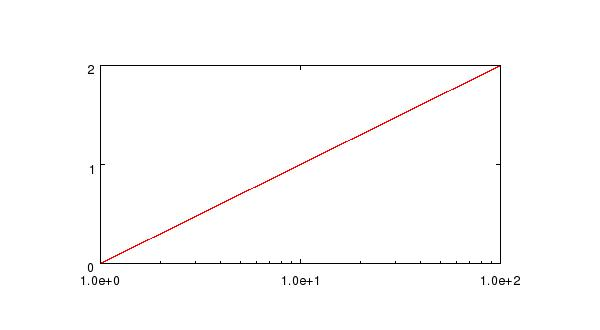
\includegraphics[width=8cm]{semilogx2}}

